\documentclass{article}

\usepackage{graphicx}

\author{Nic Hollingum - 308193415}
\title{Computer and Network Security - Assignment 1}

\begin{document}
\maketitle

\section{DES}
\subsection{DESV}
First we note the dependancy between $k$ and $k_1$.
If we are able to break $k$ we are immediately able to break $k_1$ by xoring a single plain/cipher pair with the encryption of only $k$:

$(DES_k (m) \oplus 0) \oplus (DES_k (m) \oplus k_1) = 0 \oplus k_1 = k_1$

In order to find $k$ we need to perform the DES cracking by somehow removing $k_1$ from the problem.
Again we require only a few plain/cipher pairs (2).
We Note that be xoring the ciphertext we can strip $k_1$ from the output:

$(DES_k (m_1) \oplus k_1) \oplus (DES_k (m_2) \oplus k_1) = DES_k (m_1) \oplus DES_k (m_2)$

Then we simply find the $k$ for which this holds.
This requires strictly twice the number of encryptions/decryptions to normally brute force DES, since we must encrypt 2 messages each check.
On average this means $O(2^{56})$ enc/decyyptions for a key of length 56, as indeed $k$ is.
More intelligent attaks can reduce this figure.

\subsection{DESW}
Breaking this ``enhanced'' DES requires little more effort than regular DES.
First we note that if we had $k$ we can instantl gain $k_1$ by decrypting one of our ciphertexts and xoring that with its plain pair.
However this has to be true for all of our plain/cipher pairs, so we know something about $k_1$ even without knowing $k$.
Namely, when we decrypt pair i or j with k: $DES_k (c_i) \ne m_i$ but, $DES_k (c_i) \oplus DES_k(c_j) = m_i \oplus m_j$.
Or more intuitively, when we have the right $k$, every plaintext pair will be just as different from the decryption as each other.

Thus we have our algorithm for breaking DESW.
We brue force $k$, and compare the difference between the decryption of one ciphertext and the decryption of another.
If the 2 differences are not the same, then $k$ was not chosen correctly, and we continue.
Otherwise, we have chosen the correct $k$.
Now $k_1$ is easily retrieved: $DES_k (c_i) \oplus m_i = k_1$.

\section{Hash Functions}

\subsection{Ciphers using Hash Functions}

\begin{figure}[htb]
\begin{center}
\leavevmode
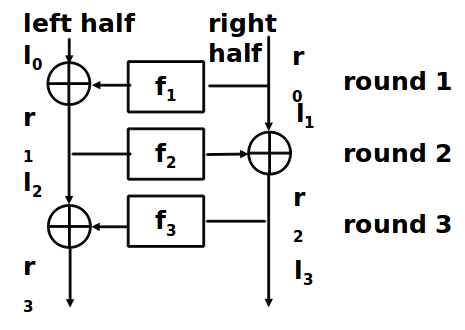
\includegraphics[width=0.4\textwidth]{feistel.png}
\end{center}
\label{fig:vortrap}
\end{figure}

This is a Feistel network, as discussed in lectures/textbooks.
This particular image was taken from Lecture slides.
This network can be used to create block ciphers using normally non-reversible functions, in our case hash functions.

We are able to decrypt this normally one-way function because we never fully hashed the input, only half at a time (for each block).
We are able to use the most recently un-hashed half in order to work out what the result would have been, the net result is to peel off a single layer of hashing from the block, at which point we can do the same for the blocks reversed, and so on until we have the original block.

\section{Protocol Analysis}


\section{Protocol Design}


\end{document}
